\centering
\subfloat[Zoo - DG]{
\begin{tikzpicture}
\begin{axis}[
ybar,
bar width=20pt,
enlargelimits=0.15,
ylabel={time in seconds},
symbolic x coords={MinCover, Maier, Duquenne},
xtick=data,
nodes near coords,
nodes near coords align={vertical},
]
\addplot[midnight, fill=clouds!80!white]
	 coordinates {(MinCover, 0.0005) (Maier, 0.0005) (Duquenne, 0.0005)};
\addplot[midnight, fill=belize!30!white] coordinates {(MinCover, 0.0004) (Maier, 0.0003) (Duquenne, 0.0002)};
\legend{DG basis, Average over 1000}
\end{axis}
\end{tikzpicture}
}
\subfloat[Zoo - Min]{
	
	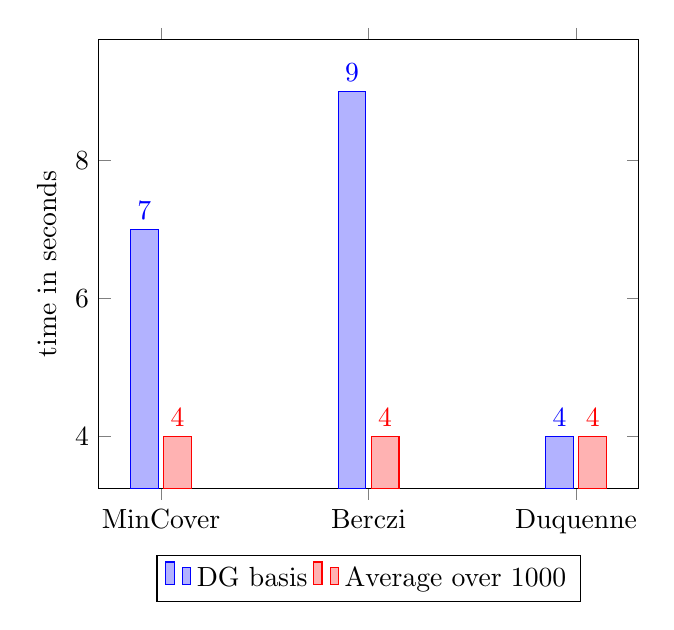
\begin{tikzpicture}
	\begin{axis}[
	ybar,
	enlargelimits=0.15,
	legend style={at={(0.5,-0.15)},
		anchor=north,legend columns=-1},
	ylabel={time in seconds},
	symbolic x coords={MinCover, Berczi, Duquenne},
	xtick=data,
	nodes near coords,
	nodes near coords align={vertical},
	]
	\addplot coordinates {(MinCover, 7) (Berczi,9) (Duquenne,4)};
	\addplot coordinates {(MinCover,4) (Berczi,4) (Duquenne,4)};
	\legend{DG basis, Average over 1000}
	\end{axis}
	\end{tikzpicture}
}